\chapter{Analyse du code}

Notre projet s'effectue dans la continuité d'un projet déjà bien entamé, ainsi, la première étape est de comprendre et d'assimiler le travail qui a déjà été effectué.

\section{Vector.cpp Vector.h}
Le fichier \textbf{Vector.cpp} permet la création de vecteurs. On y retrouve un constructeur pour les vecteur de deux dimensions et un deuxième pour les vecteurs de trois dimensions.

\begin{lstlisting}
//Exemple d'un des constructeurs :vecteurs en 2 dimensions
Vec2D::Vec2D(double a_x, double a_y)
      :x(a_x)
      ,y(a_y)
    {}
\end{lstlisting}

Le fichier Vector.h associé contient les différentes classes mettant en places les vecteurs.

\section{Types.cpp - Types.h}
Ce code ci possède des constructeurs nécessaires pour la mise en place des données liés aux particules. Nous avons :
\begin{itemize}
    \item Un constructeur à vide des particules
    \item Un constructeur de particules avec une initialisation par 2 valeurs
    \item Un constructeur utilisant la structure d'une particule situé dans le Types.h
    \item Un constructeur servant d'overload, c'est-à-dire qu'elle spécifie plusieurs fonctions possédant le même nom
    \item Une fonction permettant la réinitialisation à 0 de nos données de particules
    \item Une fonction booléenne vérifiant si une donnée de particule est vide
\end{itemize}

Voici par exemple, le constructeur à vide de particules
\begin{lstlisting}
\\Constructeur à vide de ParticleData */
ParticleData::ParticleData()
  :m_pState(NULL)
  ,m_pAuxState(NULL)
{}
\end{lstlisting}

Quand au fichier Types.h, on y retrouve différentes structures :
\begin{itemize}
    \item \textbf{PODState} pour la position et la vitesse d'une particule
    \item \textbf{PODAuxState} pour la masse d'une particule
    \item \textbf{PODDeriv} pour la vitesse et l'accélération d'une particule
    \item \textbf{ParticleData} définissant une particule

\end{itemize}
\newpage
\section{ModelNBody.cpp - ModelNbody.h}
Ce fichier contient les fonctions permettant la création de notre modèle à N-corps. Nous avons ainsi :
\newline
\begin{itemize}
    \item Une classe permettant la création de notre modèle à N-corps. Il y figure un ensemble de donnée comme par exemple la masse du Soleil ou encore la constante gravitationnelle
    \item Un destructeur de la classe précédente, dans le but de libérer l'espace alloué par notre classe
    \item une fonction définissant la région d'étude
    \item une fonction obtenant le temps des étapes
    \item une fonction récupérant la région d'étude lors de la visualisation
    \item une fonction récupérant le centre de masse
    \item une fonction permettant d'obtenir la direction de la caméra et une autre sa position lors de la visualisation
    \item Une fonction récupérant l'état initial de la simulation
    \item une fonction permettant de calculer la vitesse orbitale d'une particule par rapport à une autre particule
    \item une classe permettant la reintialisation du modèle à N-corps
    \item une classe qui initialise la simulation du modèle
    \item une autre classe qui initialise la simulation du modèle mais cette fois avec seulement 3 particules
    \item une classe permettant l'initialisation de black holes (=trou noir) accompagné de particules aléatoires
    \item une classe permettant la mise en place de l'arbre(cette notion d'arbre se clarifiera par la suite)
    \item une classe qui sert à obtenir le noeud racine de l'arbre
    \item Une classe récupérant les différents noeud
    \item une classe permettant de régler thêta et une autre classe le récupérant.Thêta est une variable qui va être utiliser lors de la mise en place de l'algorithme de Barnes-Hut
    \item une classe récupérant la masse des particules
    \item une classe calculant l'accélération et la vitesse sur chaque particule du modèle
    \item une fonction booléenne qui permet de savoir lorsque la mise en place du modèle est terminé
\end{itemize}

Par exemple, voici le destructeur du modèle à N-corps
\begin{lstlisting}
ModelNBody::~ModelNBody()
{
  delete m_pInitial;
  delete m_pAux;
}

\end{lstlisting}
Quant au ModelNbody.h , elle contient la classe permettant le traitement du modèle à N-corps

\section{BHTree.cpp - BHTree.h}
Ce fichier permet la création de fonction et de classe agissant sur un arbre. Un arbre est une structure contenant des informations(ici les particules) situés dans des éléments qu'on appelle noeuds.
\newline
On retrouve ainsi dans ce fichier la création et la reintilisation de l'arbre, des fonctions booléenne nous indiquant la racine (= noeud initial) de l'arbre, si un noeud est externe (=noeud sans descendant) ou encore si deux noeuds sont trop proche de l'un de l'autre. Des fonctions permettant d'obtenir les coordonnées du bord supérieur et inférieur d'un noeud, son centre de masse et sa variable thêta y sont définit.\newline
S'y trouve aussi une fonction permettant de récupérer le nombre de particule situé dans les noeud et une autre nous indiquant le nombre des noeuds non assignés.\newline
Une fonction calcule l'accélération causé par la gravitation d'une particule sur une autre et une autre calcule la force exercé par un noeud sur une particule.
\newpage
Quand au BHTree.h, on y retrouve une classe implémentant l'arbre de Barnes-Hut avec un seul noeud.
Par exemple dans cete classe, on retrouve plusieurs données situé dans un noeud comme le montre l'extrait de code suivant :
\begin{lstlisting}
  double m_mass;               // Masse de toutes les particules situés dans un noeud
  Vec2D m_cm;                  // Centre de masse
  Vec2D m_center;              // Centre d'un noeud
\end{lstlisting}

\section{Les intégrateurs}
Le code contient également un fichier dans lequel seront écrits les différents intégrateurs permettant de calculer les vitesses et positions de chaque particules. Pour l'instant, seul un simple intégrateur d'Euler est implémenté. 

\section{La visualisation}
Des classes et méthodes gérant l'affichage des particules est aussi implémenté à partir des bibliothèques SDL et OpenGL, ce qui nous permet de pouvoir nous concentrer sur les calculs qui doivent être effectués.

%inclusion d'une mage dans le document
\begin{figure}[!h]
\begin{center}
%taille de l'image en largeur
%remplacer "width" par "height" pour régler la hauteur
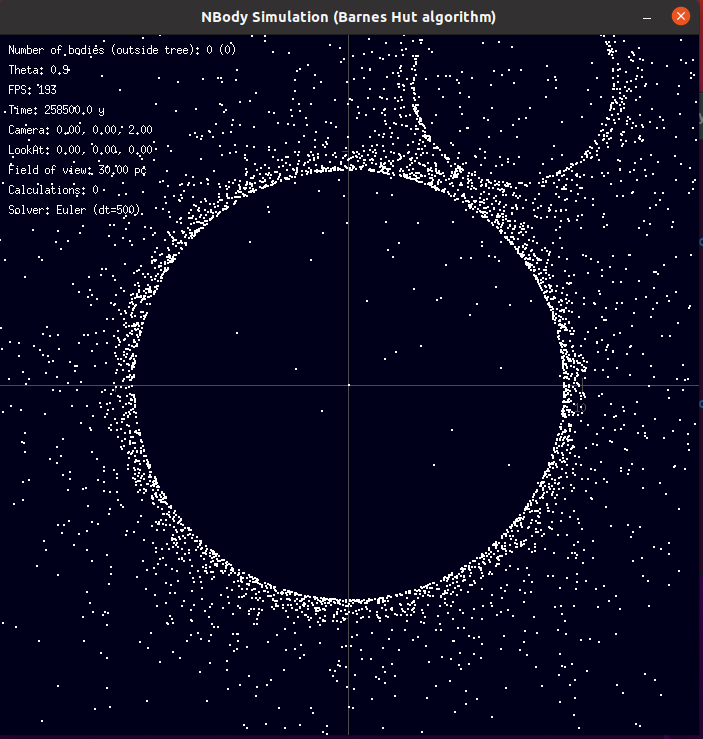
\includegraphics[width=13cm]{aff.png}
\end{center}
%légende de l'image
\caption{Visualisation (aucun calcul effectué)}
\end{figure}
 
